\section{Aktivitätsdiagramm}

\begin{tcolorbox}[title=Einsatzbereich]
    Aktivitätsdiagramme können in \textit{allen Phasen} des Softwareentwicklungsprozesses eingesetzt werden:

    \begin{itemize}
        \item \textbf{Analyse}: Modellierung von Geschäftsprozessen
        \item \textbf{Anforderung}: Verhalten von Anwendungsfällen
        \item \textbf{Entwurf}: Darstellung von Systemverhalten, Vorlage zur Umsetzung in Sourcecode
        \item \textbf{Implementierung}: Darstellung komplexer Algorithmen
        \item \textbf{Testphase}: Ableitung von Testfällen
    \end{itemize}

    \noindentIn
    In \textbf{Aktivitätsdiagrammen} werden \textbf{Aktivitäten} modelliert, die \textbf{Aktivitätsknoten} und \textbf{Aktivitätskanten} enthalten.\\

    \noindent
    \textbf{Aktivitätsknoten} existieren in drei Ausprägungen:

    \begin{itemize}
        \item \textbf{Ausführbare Knoten}: Knoten, die Tätigkeiten ausführen, also bspw. eine Aktion.
        \item \textbf{Objektknoten}: Knoten, die Daten speichern können (bspw. Puffer, Datastore).
        \item \textbf{Kontrollknoten}: Knoten, die den Ablauf beeinflussen, bspw. Verzweigungen.
    \end{itemize}

    \noindent
    Parallele Abläufe lassen sich mit Aktivitätsdiagrammen sehr übersichtlich darstellen.
\end{tcolorbox}


\begin{figure}
    \centering
    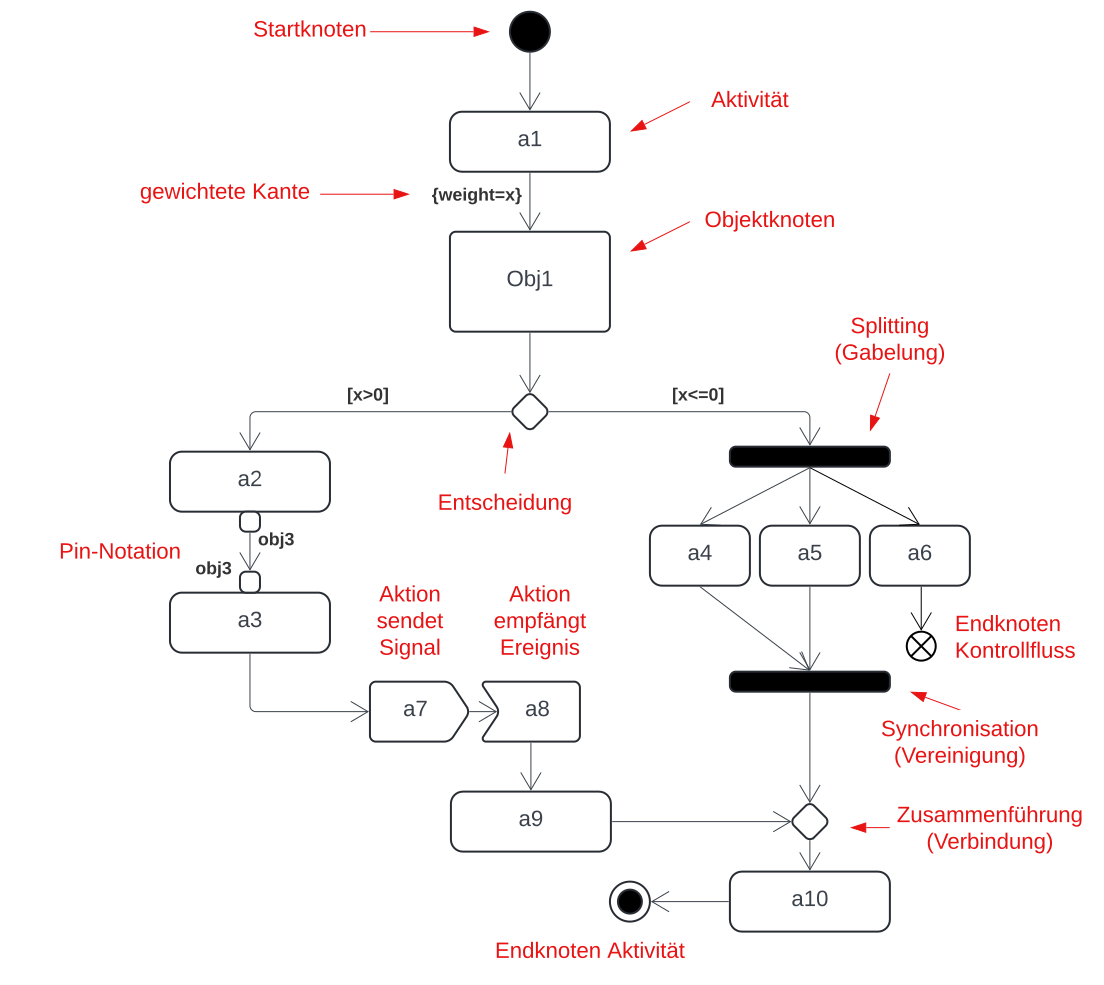
\includegraphics[scale=0.35]{part three/Aktivitätsdiagramme/img/aktivitätsdiagramm-notation}
    \caption{Verschiedene Notationen für Elemente in einem Aktivitätsdiagramm. (Quelle: in Anlehnung an \cite[326, Abb. 6.9-16]{Bal05})}
    \label{fig:aktivitätsdiagramm-notation-cc}
\end{figure}